\chapter{Model of System}
The overall goal is to ensure that the structure will meet present and likely future demands on it.
\section{Architecture Model}
An architectural model provides the definition of what are components, structures of the system and functions associated with them. There are different types of processes:
\begin{itemize}
    \item Client
    \item Server
    \item Peer
\end{itemize}
Architectural models can be classified in client-server or peer processes. A \textbf{client-server architecture} can be based on layers or tiers.
\begin{itemize}
    \item A \textbf{layer architecture} splits a complex system into a \textbf{number of layers}, in which each level uses functions of the below layer and in turn, it will offer other services to the upper levels.
    \item \textbf{Tired architectures} are complementary to layering. Whereas layering deals with the vertical organisation of services into layers of abstraction. This technique is most commonly associated with the \textbf{organisation of applications and services}. Each tier level is used as a level of abstraction
\end{itemize}

\subsection{Client - Server}
Client-server architecture is the most common and based on the idea that there are some processes, called \textbf{clients}, that ask for resources and special processes, called \textbf{servers}, that serve requests and rely on them. When the client submits a request it waits until it receives the result. The
time between send a request and receive the corresponding response is called \textit{response time}.
\begin{figure}[!h]
            \centering
            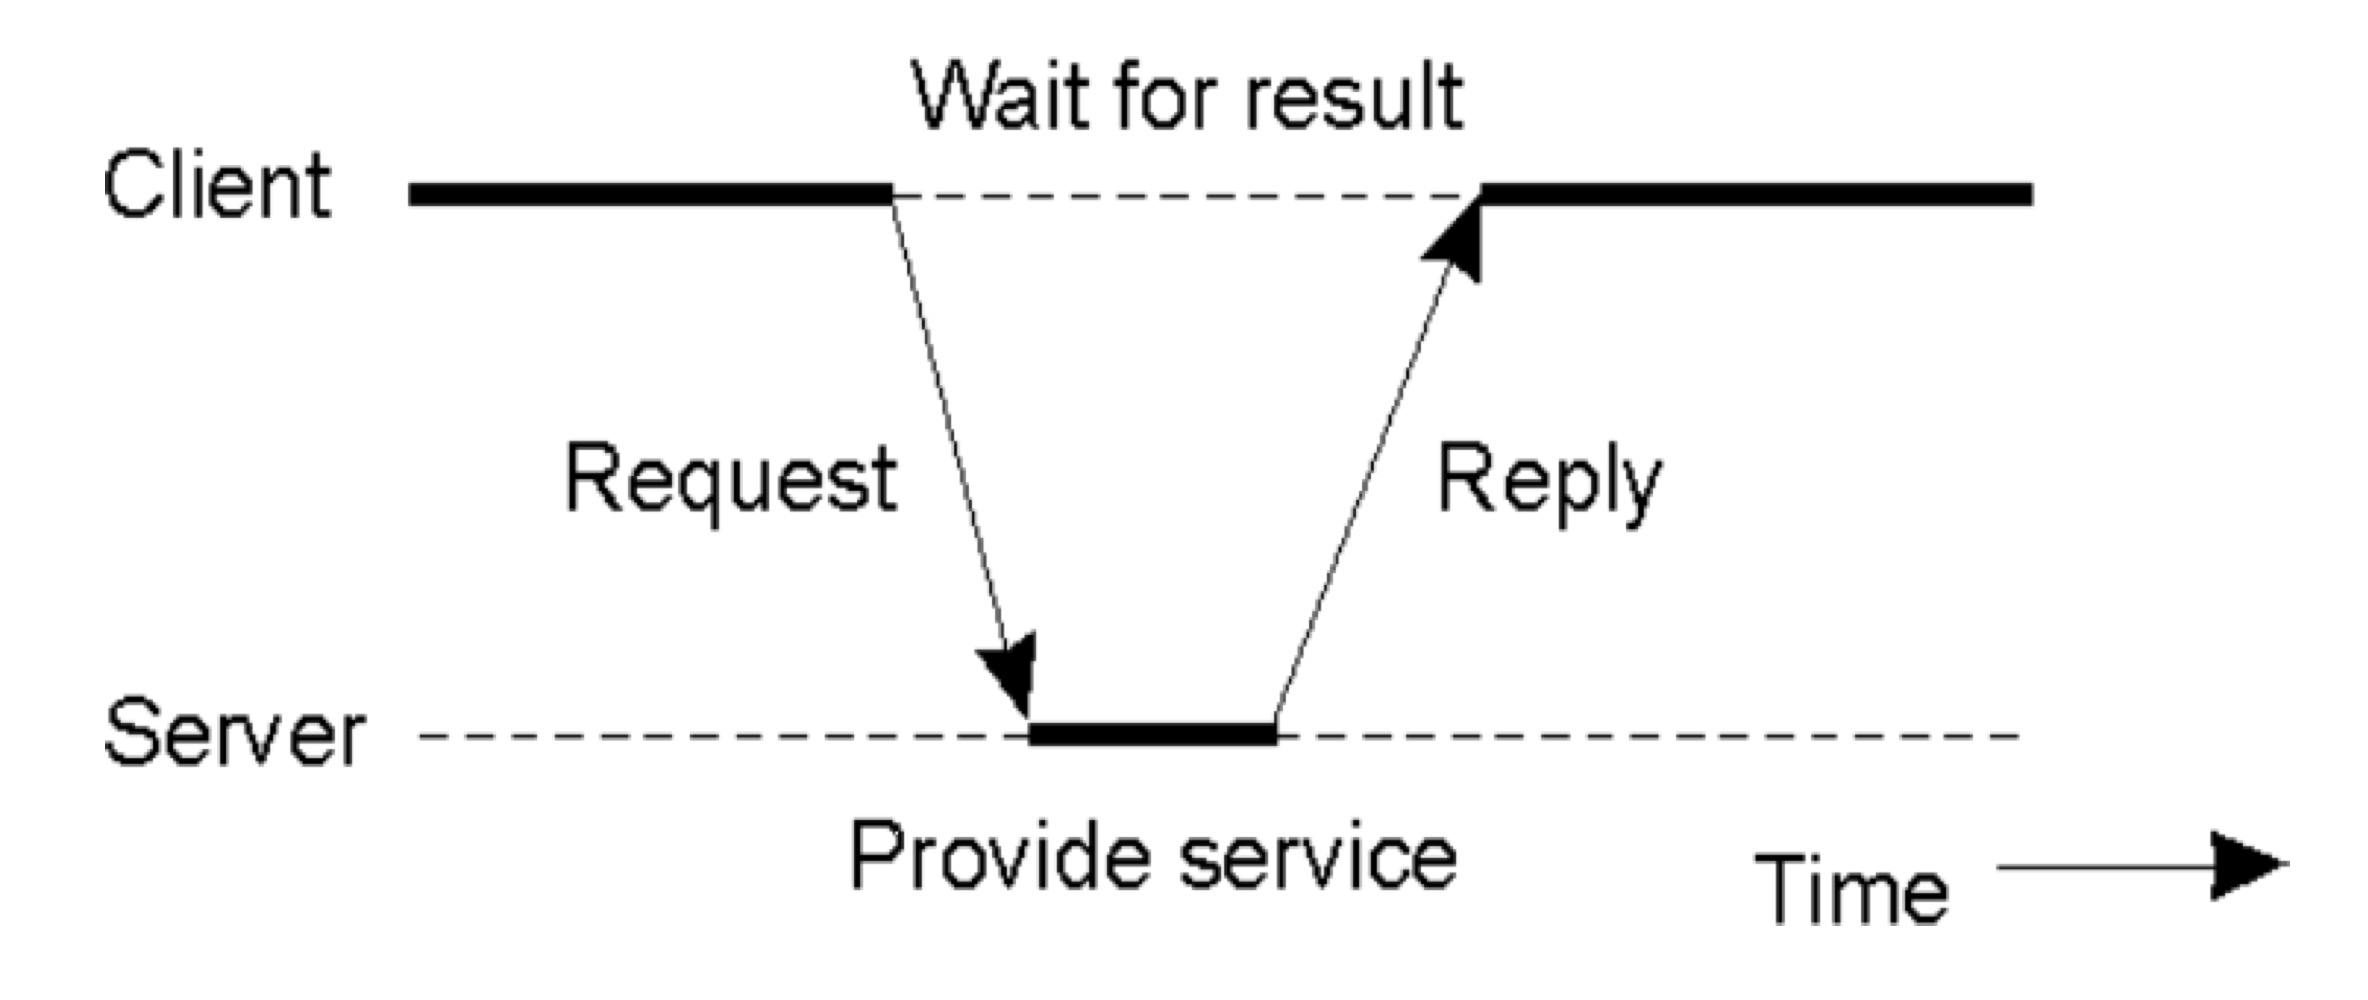
\includegraphics[width=.7\linewidth]{images/modelOfSystems/SingleTierArchitecture.jpeg}
            \caption{Client - Server Single Tier Architecture}
    \end{figure}
    \newpage
Considering a more complicated architecture with two tiers, response time can be greater, since also the server has to wait for the required resource.

\begin{figure}[!ht]
            \centering
            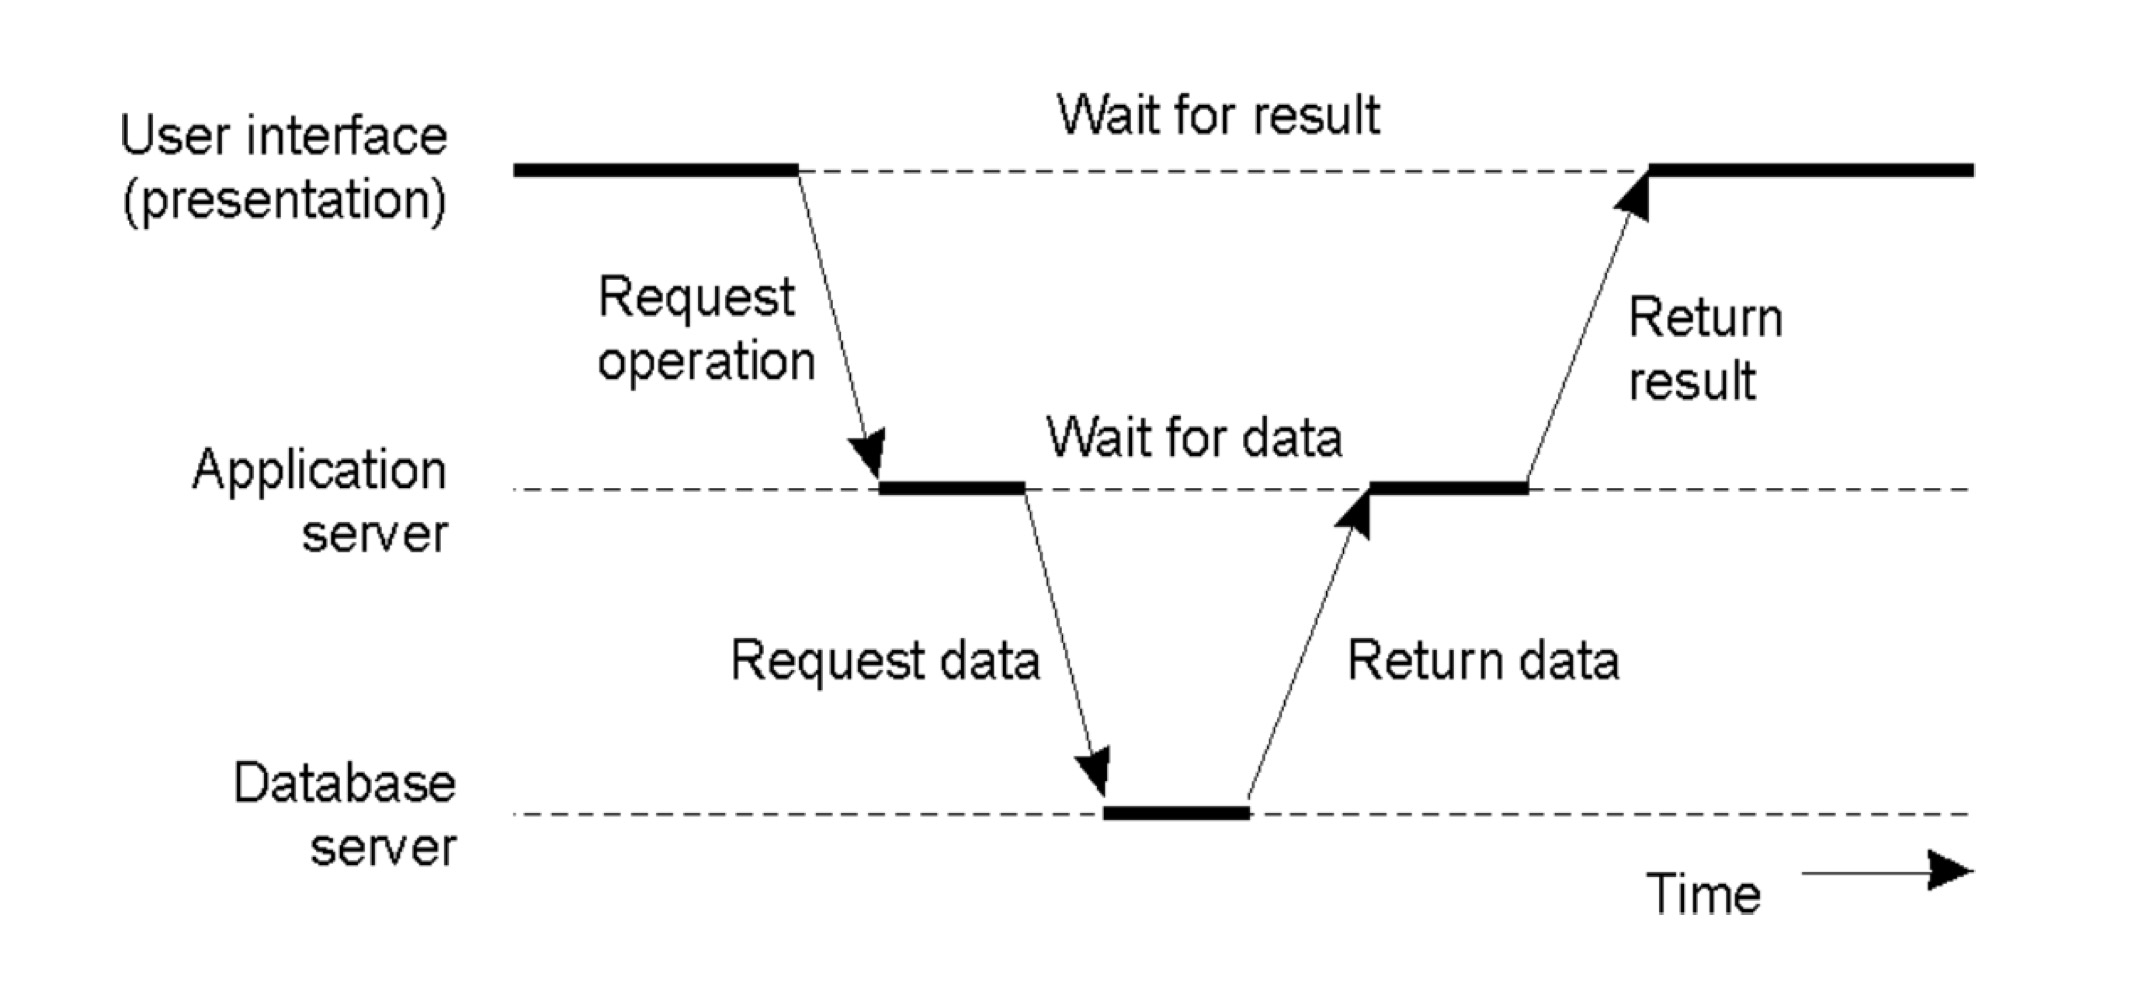
\includegraphics[width=.7\linewidth]{images/modelOfSystems/MultiTierArchitecture.jpeg}
            \caption{Client - Server Multi Tier Architecture}
    \end{figure}
Client-Server architecture can be composed of a \textbf{set of servers} that provide the same services and they can interact to reduce the load of each server. Respecting the previous simple model, with only one server, these kinds of architectures are also fault tolerant, since if at least one is up the system can provide response.
Some of these architectures introduce a new component called \textbf{proxy}, used to \textbf{reduce the traffic and provide cache functionalities}. The proxy pattern is famous to to support location transparency in remote procedure calls or remote method invocation.

\subsection{Peer-To-Peer}
Peer-to-peer systems represent a \textbf{paradigm} for the construction of distributed systems and applications in which data and computational resources are contributed by \textbf{many hosts} on a network. Processes can be everywhere, but they have to cooperate in order to solve problems of consistency of the resources and to synchronize their actions. 

In this architecture, \textbf{all the processes involved in a task or activity play similar roles}, interacting cooperatively as peers without any distinction between client and server processes or the computers on which they run.
\newpage
\begin{figure}[!h]
            \centering
            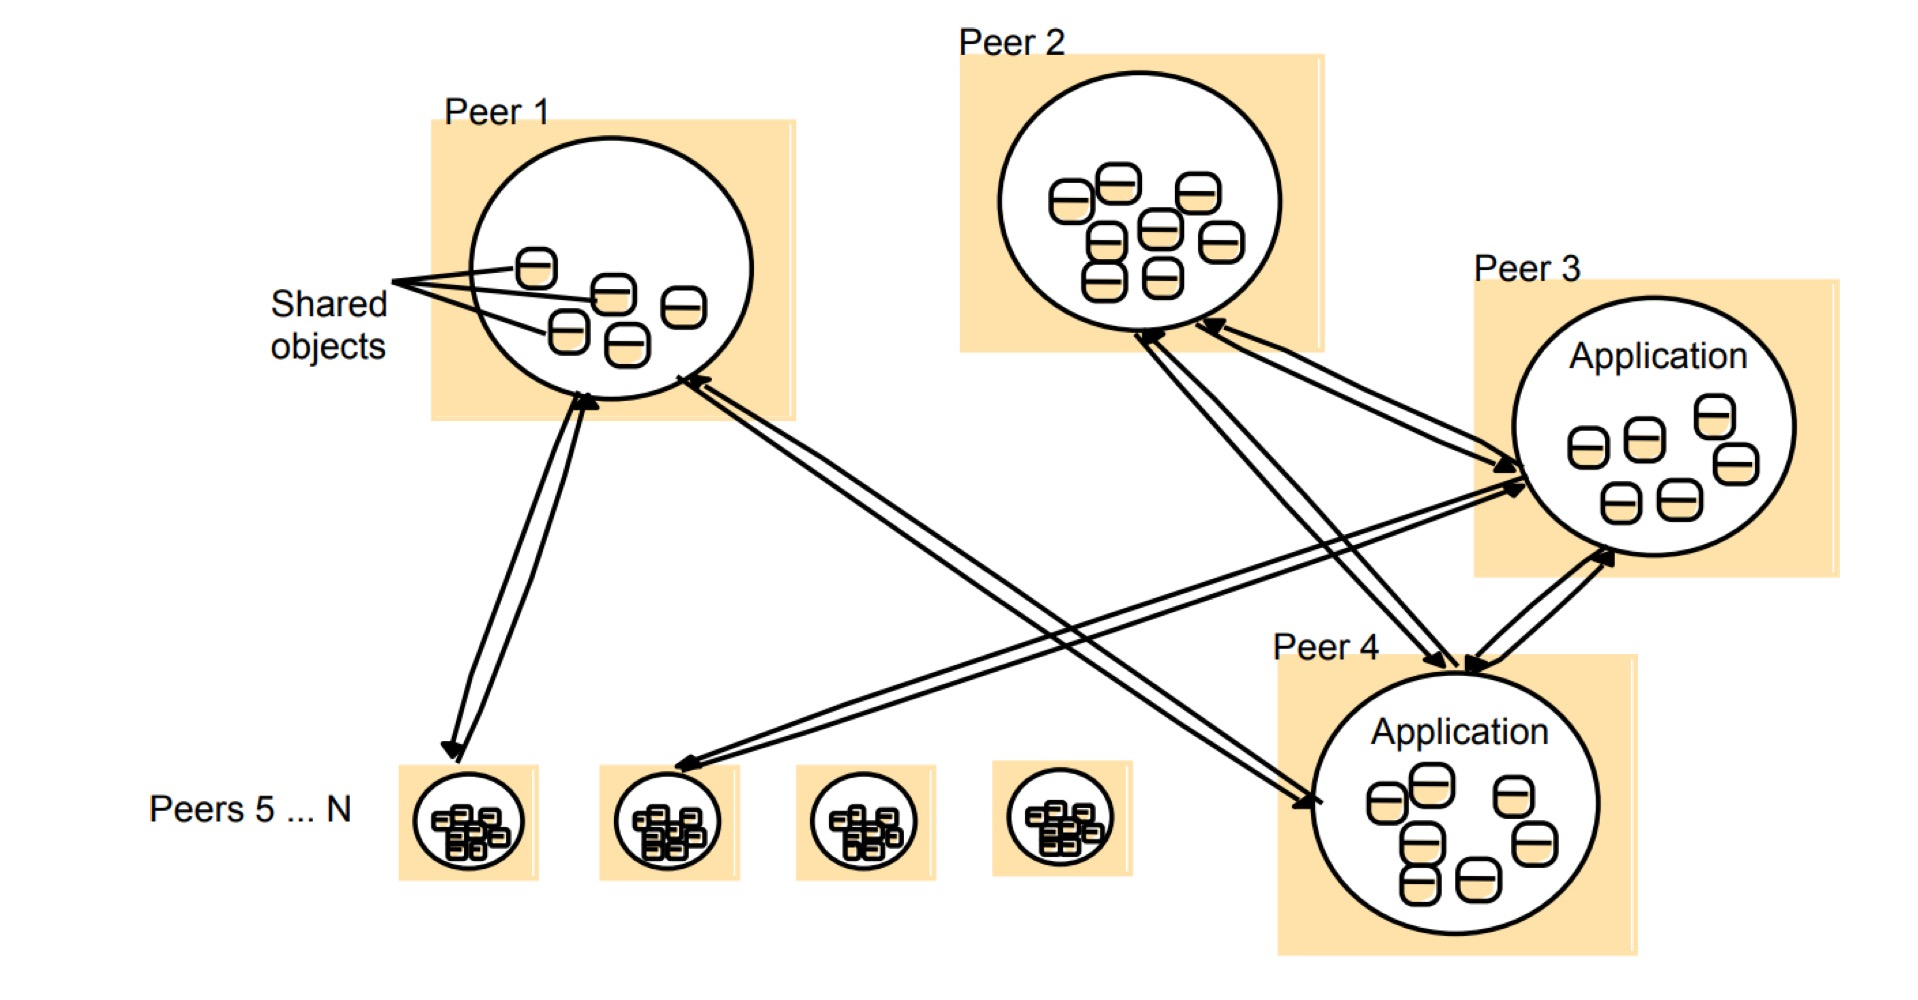
\includegraphics[width=.7\linewidth]{images/modelOfSystems/Peer-to-PeerArchitecture.jpeg}
            \caption{Peer-to-Peer Architecture}
    \end{figure}
A key problem for peer-to-peer systems is the \textbf{placement of data objects across many hosts} and subsequent provision for access to them in a manner that balances the workload and ensures availability without adding undue overheads.

\subsection{Variants of Client - Server Model}
Could be \textbf{mobility} of the node, of the code (program can be moved) or data.
\begin{itemize}
    \item Like \textbf{Applets}, which are a well-known and widely used example of mobile code – the user running a browser selects a \textbf{link to an applet} whose code is stored on a web server; the \textbf{code is downloaded} to the browser and runs there. 
    
    An advantage of running the downloaded code locally is that it can give a \textbf{good interactive response} since it does not suffer from the delays or variability of bandwidth associated with network communication.
    
    When a client requests something from the server, the reply given by the server is an applet code that will be executed from the client hardware.
    \item A \textbf{Mobile Agent} is a running program that travels from one computer to another in a network carrying out a task on someone’s behalf (comportamento), such as collecting information, and eventually returning with the results.
\end{itemize}

\section{Fundamental Model}
All of the previous models are composed of processes that communicate with one another by sending messages over a computer network. All of the models share the design requirements of achieving the performance, correctness and reliability characteristics of processes and networks and ensuring the security of resources in the system. Fundamental models decide to focus their attention to some particular aspects:
\begin{itemize}
    \item \textbf{Interaction Models:} \textit{how process interact.}Like using message passing, moreover we have to consider also the delay time.
    \item \textbf{Faults Models:} focus the attention on the \textit{problem of possible faults of the system.} They define and classify faults, providing a basis for the analysis of their potential effects and for the design of systems that are able to tolerate faults of each type while continuing to run correctly.
    \item \textbf{Security Model:} a distributed system can be \textit{exposed to attack by both external and internal agents.} Security model defines and classifies the forms that such attacks may take, providing a basis for the analysis of threats to a system and for the design of systems that are able to resist them.
    \item \textbf{Performance Model}
\end{itemize}

\subsection{Interaction Models}
Messages are transmitted between processes to transfer information between them and to coordinate their activities. Each process has its own state, consisting of the set of data that can access and update, including the variables in its program. The state belonging to each process is completely private – that is, it cannot be accessed or updated by any other process.
\begin{itemize}
    \item \textbf{Latency:} the delay between time of starting transmission and time starting to receive the message by receiver
    \item \textbf{Band:} the total amount of information that can be transmitted in the network in a given time.
    \item \textbf{Jitter:} variation in the time taken to deliver a series of messages. Measurement relevant for streaming and multimedia purpose.
    \item \textbf{Lack of Global Time} There is not a unique clock but each process has its own clock and they usually are not synchronised. One solution can be to implement a virtual clock used by each process to verify the current state of the system.
    \item A distributed system can be also classified as \textbf{synchronous} or \textbf{asynchronous}.
    \begin{itemize}
        \item In synchronous systems processes are synchronized and so it is easier to develop communication protocols
        \item Instead, asynchronous systems are not bounded, so it is necessary to develop different strategies to provide communication protocols
    \end{itemize}
\end{itemize}
\begin{figure}[!h]
            \centering
            \includegraphics[width=.7\linewidth]{images/modelOfSystems/ReceiversInDIfferentOrder.jpeg}
            \caption{Organization of cloud computing - levels of services - Example
}
    \end{figure}
\newpage

\subsection{Fault Models}
In a distributed system \textbf{both processes and communication channels may fail.} The failure model defines the ways in which failure may occur in order to provide an understanding of the effects of failures.
\begin{figure}[!h]
            \centering
            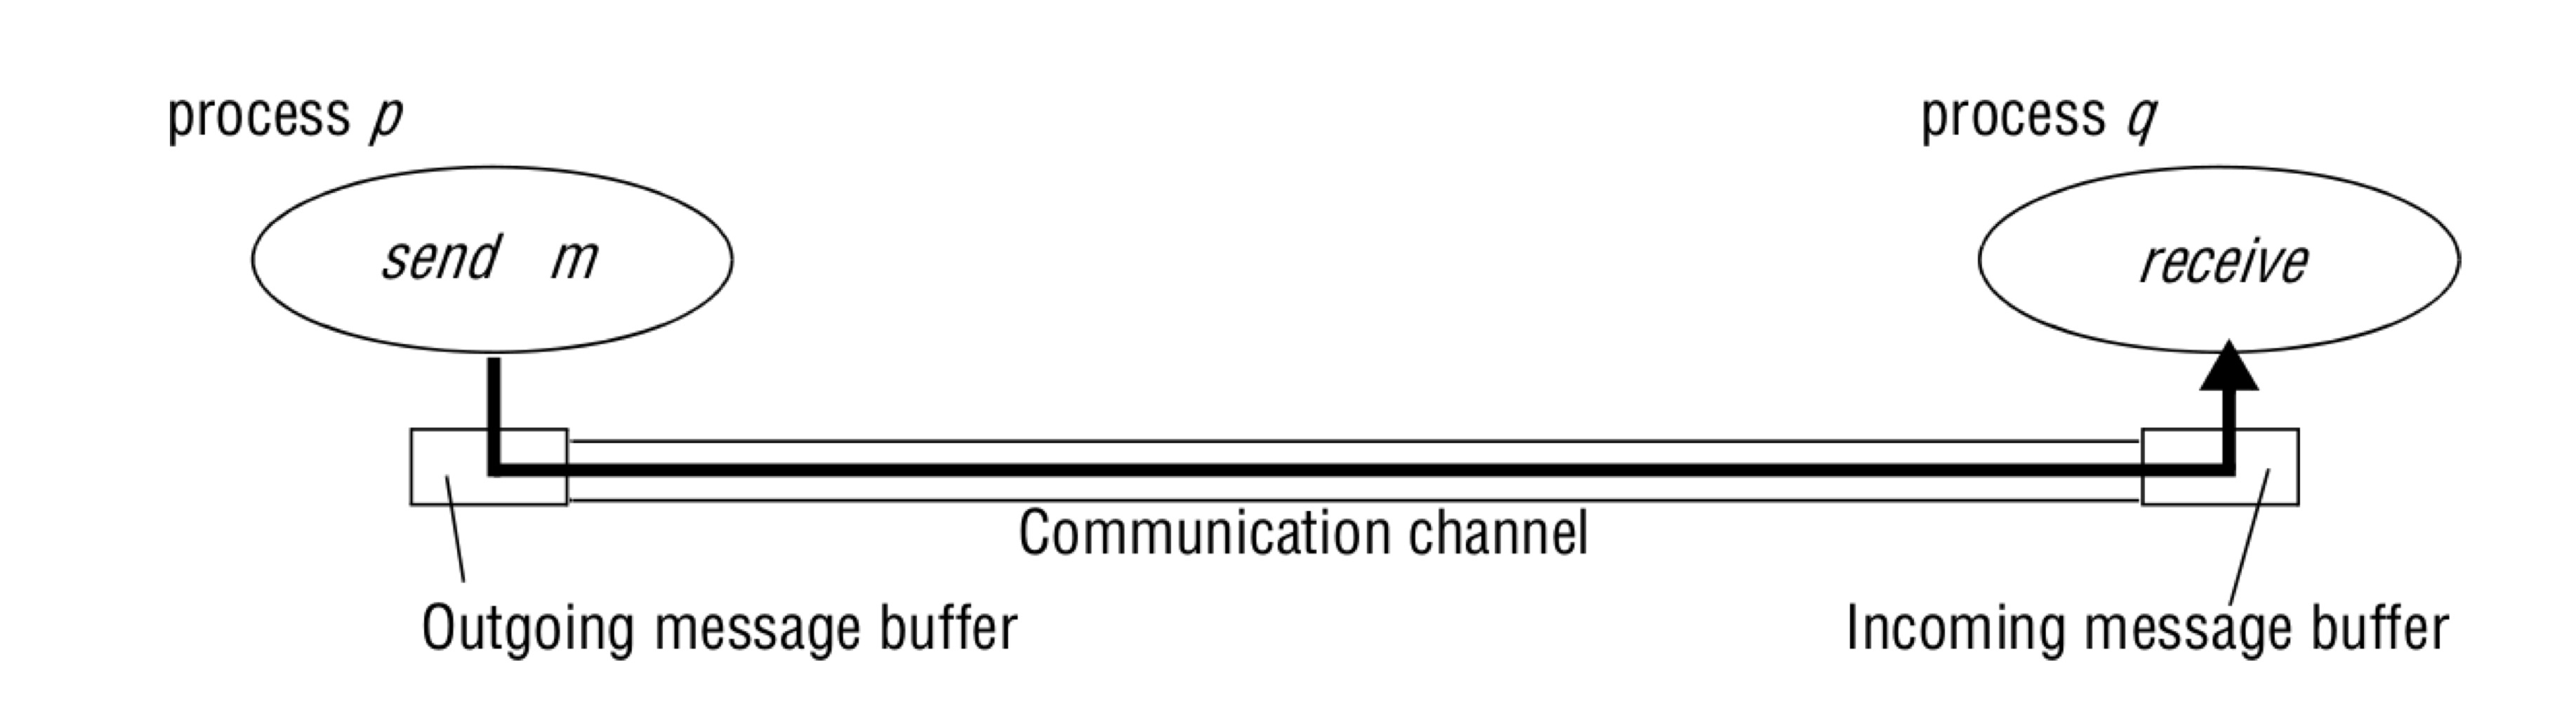
\includegraphics[width=.7\linewidth]{images/modelOfSystems/ArbitraryFailure.jpeg}
            \caption{Organization of cloud computing - levels of services - Example
}
    \end{figure}
There are different types of failure:
\begin{figure}[!h]
            \centering
            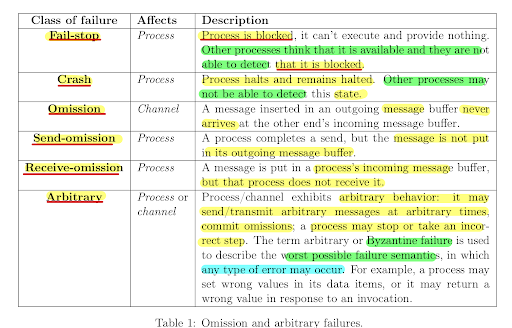
\includegraphics[width=.8\linewidth]{images/modelOfSystems/table1.png}
    \end{figure}
    
Other kinds of failure are called \textbf{timing failures} and they are associated only to synchronous
systems, that have the constraint of time bounds.
\begin{figure}[!h]
            \centering
            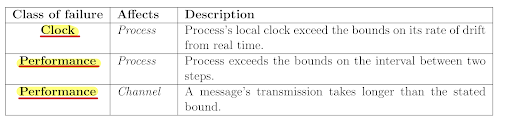
\includegraphics[width=.8\linewidth]{images/modelOfSystems/table2.png}
    \end{figure}

\subsection{Security Models}
A distributed system can be interested in possible attacks, so it is necessary to develop systems and strategies for \textbf{authentication, cryptography and for maintaining integrity and security of the entire system and resources.}
\begin{figure}[!h]
            \centering
            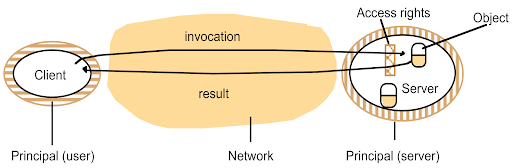
\includegraphics[width=.7\linewidth]{images/modelOfSystems/UserProcessWithAutority.jpeg}
            \caption{User Process with Autority}
    \end{figure}
\begin{figure}[!h]
            \centering
            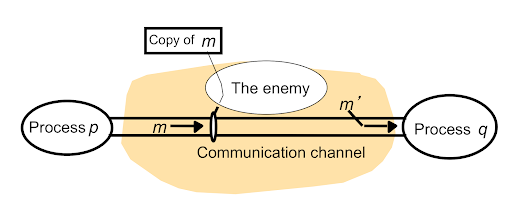
\includegraphics[width=.7\linewidth]{images/modelOfSystems/CommunicationAttack.jpeg}
            \caption{Communication Attack}
    \end{figure}
There are different type of attack that a enemy could take:
\begin{itemize}
    \item \textit{Eavesdropping:} obtain private or secret information
    \item \textit{Masquerading:} assuming the identity of another user
    \item \textit{Message tampering:} altering the content of messages in transit (ma in the middle attack)
    \item \textit{Replaying:} storing secure messages and sending them at a later date/time
    \item \textit{Denial of Services:} flooding a channel or other resource, denying access to others
\end{itemize}

\begin{figure}[!h]
            \centering
            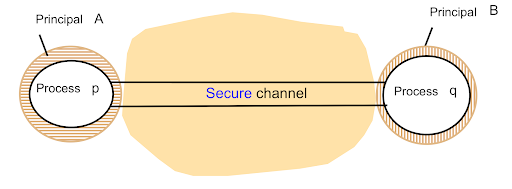
\includegraphics[width=.7\linewidth]{images/modelOfSystems/SecureChannel.jpeg}
            \caption{Secure Channel
}
    \end{figure}
A secure channel must take into account these security features:
\begin{itemize}
    \item Cryptography and shared secret information like key
    \item Authentication based on proof of ownership of secret
    \item Privacy and integrity
    \item Use of timestamp to avoid messages from being recorded
    \item VPN, SSL, SFTP
\end{itemize}

\subsection{Performance Models}
The most important performance indexes are:
\begin{enumerate}
    \item Throughout (X)
    \item Mean Response Time (R)
    \item Utilization (U)
\end{enumerate}
In this section we focus in three main cases:
\subsubsection{Performance models with basic queue}
This is a simple queried model for a centralised system where we have three general assumptions:
\begin{itemize}
    \item Independence job
    \item Exponential times 
    \item Infinite buffer queue
\end{itemize}
\begin{figure}[!h]
            \centering
            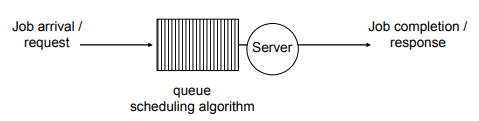
\includegraphics[width=.7\linewidth]{images/modelOfSystems/PerformanceModelsWithBasicQueue.png}
            \caption{Organization of cloud computing - levels of services - Example
}
    \end{figure}

Now we introduce two type of measure:
\begin{itemize}
    \item Job arrival rate: 		$\lambda$ 	request/sec
    \item Service rate: 		    $\mu$ 	request/sec
\end{itemize}

\subsubsection{Performance models with basic queue and one server}
This is a basic queuing (fare la fila) model for a centralized system where we have exponential and independence assumptions.
\begin{figure}[!h]
            \centering
            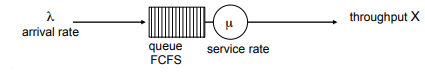
\includegraphics[width=.7\linewidth]{images/modelOfSystems/PerformanceModelsWithBasicQueueAndOneServer.png}
            \caption{Performance models with basic queue and one server
}
    \end{figure}
\textit{Proprieties:}
\begin{itemize}
    \item The model is stable if \(\lambda < \mu\)
    \item We define the traffic intensity \(p = \lambda / \mu\)
    \item Utilization (U): 			\(U = p\)
    \item Mean Response Time (R):	\(R = 1 / (\mu - \lambda) sec\)
    \item Throughput (X):		    \(X = \lambda \frac{req}{sec}\)
    \item Mean Queue Length (N):	\(N =  p / (1 - p)\)
\end{itemize}
Queue Length probability: \(\pi_i = p^i\times (1 - p)    i \geq 0\) probability of i jobs in the systems
\begin{figure}[!h]
            \centering
            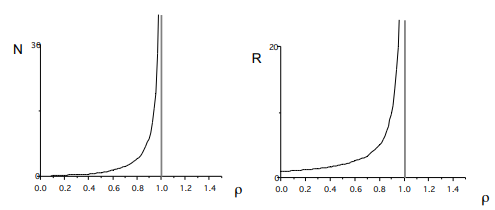
\includegraphics[width=.7\linewidth]{images/modelOfSystems/meanJob.png}
            \caption{Organization of cloud computing - levels of services - Example
}
    \end{figure}



\subsubsection{Performance model with queue and multiple server}
Basic queuing model for a system with multiple servers (processors), where we have the exponential and independent assumptions. Here we have to introduce an additional type of measure, so in summary we have:
\begin{itemize}
    \item Job arrival rate: 				\(\lambda\) 	request/sec
    \item Service rate: 				    \(\mu\) 	request/sec
    \item Number of servers per processors: 	(m \(\#\) servers) / processors
\end{itemize}
\begin{figure}[!h]
            \centering
            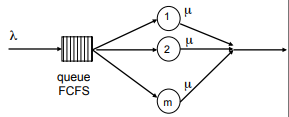
\includegraphics[width=.7\linewidth]{images/modelOfSystems/PerformanceModelWithQueueAndMultipleServer.png}
            \caption{Performance model with queue and multiple server
}
    \end{figure}


\textit{Proprieties:}
\begin{itemize}
    \item The model is stable if \(\lambda < m \times \mu\)
    \item We define the traffic intensity \(p = \lambda / (m \times\mu)\)
    \item Utilization (U): 			\(U = p\)
    \item Mean Response Time (R):	\(R = N / X\) sec
    \item Throughput (X):		    \(X = \lambda \frac{req}{sec}\)
    \item Mean Queue Length (N):	\(N = (m \times p) + (\pi_m \times p) / (1 - p)^2\)
\end{itemize}
Queue Length probability: 
\begin{enumerate}
    \item \(\pi_i = \pi_0 \times (m \times p )^i / i!\) for \(i \leq i \leq m\) probability of i jobs in the systems
    \item \(\pi_i = \pi_0 \times m^{(m)} \times p^{(i)} / m!\) for \(i > m \leq m\)
\end{enumerate}

\subsubsection{Relations of Performance Models with basic queue}
\begin{itemize}
    \item \textit{Little’s Law:} \(N = X \times R \rightarrow\) average \# of jobs in the system = throughput \(\times\) mean response time
    \item \textit{Utilization Law:} \(U = X \times S \rightarrow\) system utilization = throughput \(\times\) average service time
    \item \textit{Flow Forced Law:} \(X_k = X \times V_k \rightarrow\) throughput of a component k = system throughput \(\times\) average \# visit to component k
\end{itemize}